\ofjob{Thief}
{
	\ofquote{"I PREFER the term ”treasure hunter!"\\}{Locke}\\\\
	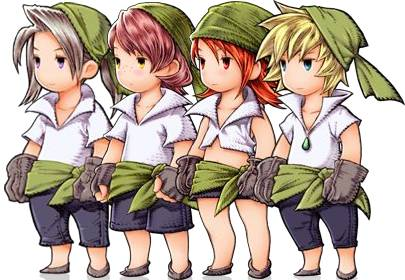
\includegraphics[width=\columnwidth]{./art/jobs/thief.jpg}\ofrow
	\accf{Thieves} are mobile melee fighters, who can quickly traverse the battlefield and are difficult
	to hit with physical attacks. 
	They excel at "borrowing" items and money from enemies and have a heightened sense for worthwhile business. 
%	One would be advised to be careful when dealing with a Thief, they always have one more trick up their
%	sleeve than you would expect.
}
{Dagger}{Light Armor}{
	Level 1: & HP +20 & MP~+19 & AGI~+4 \\
	Level 2: & HP~+5  & MP~+10  & STR~+1 & DEF~+1 \\
	Level 3: & \multicolumn{3}{l}{Archetype Attribute Bonus} \\
	Level 4: & HP~+10 & MP~+5  & STR~+1 & DEF~+1 \\
	Level 5: & HP~+10 & MP~+10 & STR~+1 &        \\ 
	Level 6: & HP~+5  & MP~+5  & DEF~+2 & RES~+1 \\ 
	Level 7: & HP~+10 & MP~+10 & STR~+1 &        \\ 
	Level 8: & HP~+10 & MP~+5  & RES~+2 &        \\ 
	Level 9: & HP~+5  & MP~+10 & STR~+2 &        \\ 
	Level 10:& HP~+10 & MP~+10  & DEF~+1 
}{
	\ofjobtech{Steal}{4}{0r}{Single}{Weapon}{Make a DC 7 check and "borrow" something from the target if you succeed. Roll 1d and the you get 2d times 10 Gil on 1 or 2, a Potion on a 3, a Remedy on a 4, an Ether on a 5 and a Phoenix Down on a 6. The item may also be determined in any other way by the GM.}{}{1} \ofabilitygap
	\ofjobtech{Flee}{3}{1r}{3u}{Self}{You and all allies in the target area can move twice as fast when running away from enemies for 3 rounds.}{}{2} \ofabilitygap
	\ofjobtech{Poison Dart}{6}{0r}{Single}{4u}{The target makes a DC~7 check and suffers 2d damage and one of the following Status Effects for 3 rounds upon failure: Poison, Immobile, Sleep}{}{6}\ofabilitygap
	\ofjobtech{Vanish}{8}{0r}{Single}{Weapon}{You become invisible for up to  5 rounds or until you take an action. While invisible, you gain Blink and have Advantage on all stealing related checks. Also, if you hit an Attack while invisible, you always score a Critical Hit.}{\blink}{8} \ofabilitygap
	\ofjobtech{Mirror Image}{23}{1r}{Single}{1u}{You create an exact copy of yourself. The clone lasts for up to 3 rounds and acts with you on your turn, following your command. The clone can use the same abilities except this one. You cannot create a clone while a previous one is still active.}{}{10}
}{
	\ofarchetypet{Ninja}
	{HP~+14 & MP~+11 & STR~+2}
	{\ofarchetypetecha{Throw}{2}{0r}{Single}{5u}{You throw a piece of equipment from your inventory on the target and deal an amount of damage depending on its equipment class. The damage dealt is 1d for Beginner, 2d for Advanced and 3d for Expert level equipment. You can collect all thrown objects at the end of the battle.}{}}
	{\ofarchetypepassive{First Strike}{When an ally chooses you to take the next turn, you can immediately take it instead of waiting for a turn of the opposing party.}}
	{\ofarchetypereaction{Counter Attack}{When an enemy hits you with an Attack, you can immediately make an Attack on him if he is within range.}}
	{\ofarchetypetechb{Assassinate}{14}{0r}{Single}{3u}{Move to the target and make an Attack on him. If you hit, he makes a DC~7 check and suffers KO upon failure.}{\ko}}
}{
	\ofarchetypet{Treasure Hunter}
	{HP~+10 & MP~+20 & DEF~+1 & RES~+1}
	{\ofarchetypetecha{Quick Pockets}{6}{0r}{Single}{Self}{Make an Attack after which you can immediately use an Item.}{}}
	{\ofarchetypepassive{Gilionaire}{Whenever you deal damage to an enemy, you also receive an amount of Gil equal to the damage dealt.}}
	{\ofarchetypereaction{Counter Steal}{Whenever you evade an Attack by an enemy, you can immediately use "Steal" on him without any cost.}}
	{\ofarchetypetechb{Gil Toss}{8}{0r}{Single}{5u}{Throw an amount of Gil on the target up to maximum of 100 Gil. The target suffers 1d damage for every 20 Gil thrown.}{}}
}